\documentclass[11pt, oneside]{article}  	% use "amsart" instead of "article" for AMSLaTeX format
\usepackage[margin=2.25cm]{geometry}        		% See geometry.pdf to learn the layout options. There are lots.
\geometry{letterpaper}          		% ... or a4paper or a5paper or ... 
%\geometry{landscape}        		% Activate for rotated page geometry
%\usepackage[parfill]{parskip}  		% Activate to begin paragraphs with an empty line rather than an indent
\usepackage{graphicx}				% Use pdf, png, jpg, or eps§ with pdflatex; use eps in DVI mode
								% TeX will automatically convert eps --> pdf in pdflatex	
								
%\usepackage[T1]{fontenc}
%\usepackage[utf8]{inputenc}
%\usepackage{babel}
%\usepackage{csquotes}
									
\usepackage{amssymb}
\usepackage{lineno}
\linenumbers
\usepackage{setspace}
%\doublespacing
\usepackage{authblk}
\usepackage{hyperref}
\usepackage{xcolor}

%\usepackage{pythonhighlight}

\usepackage[utf8]{inputenc}

% Default fixed font does not support bold face
\DeclareFixedFont{\ttb}{T1}{txtt}{bx}{n}{10} % for bold
\DeclareFixedFont{\ttm}{T1}{txtt}{m}{n}{10} % for normal

% Custom colors
\usepackage{color}
\definecolor{deepblue}{rgb}{0,0,0.5}
\definecolor{deepred}{rgb}{0.6,0,0}
\definecolor{deepgreen}{rgb}{0,0.5,0}

\usepackage{listings}

% Python style for highlighting
\newcommand\pythonstyle{\lstset{
language=Python,
basicstyle=\ttm,
morekeywords={self},       % Add keywords here
keywordstyle=\ttb\color{deepblue},
emph={MyClass,__init__},     % Custom highlighting
emphstyle=\ttb\color{deepred},  % Custom highlighting style
stringstyle=\color{deepgreen},
frame=none,             % Any extra options here
showstringspaces=false,
numbers=none,
numbersep=5pt,
aboveskip=20pt,
belowskip=20pt,
xleftmargin=0.5cm,
}}

% Python environment
\lstnewenvironment{python}[1][]
{
\pythonstyle
\lstset{#1}
}
{}

% Python for external files
\newcommand\pythonexternal[2][]{{
\pythonstyle
\lstinputlisting[#1]{#2}}}

% Python for inline
\newcommand\pythoninline[1]{{\pythonstyle\lstinline!#1!}}


\usepackage{natbib}

\usepackage{lipsum} 

\hypersetup{
  colorlinks,
  linkcolor={red!50!black},
  citecolor={blue!50!black},
  urlcolor={blue!80!black}
}

\author{Joseph D. Hughes}
\affil{U.S. Geological Survey, Model Support and Maintence Branch, 927 W Belle Plaine Ave, Chicago, IL, USA}
\author{Christian D. Langevin}
\affil{U.S. Geological Survey, Model Support and Maintence Branch, 2280 Woodale Dr, Mounds View, MN, USA}
\author{Scott R. Paulinski}
\affil{U.S. Geological Survey, California Water Science Center, 4165 Spruance Road, Suite 200, San Diego, CA, USA}
\author{Joshua D. Larsen}
\affil{U.S. Geological Survey, California Water Science Center, 6000 J Street, Placer Hall, Sacramento, CA, USA}
\author{David Brakenhoff}
\affil{Artesia Water, Korte Weistraat 12, Schoonhoven, Netherlands}


\begin{document}

\onecolumn

\title{Modern and Reproducible Groundwater Modeling Workflows with FloPy} 

\maketitle


\begin{abstract}

\noindent FloPy functionality has been expanded from the capabilities described in \cite{bakker2016scripting} to support the capabilities of the latest version of MODFLOW (MODFLOW 6). 

\end{abstract}

\section{Introduction}

FloPy is a popular Python package for constructing, running, and post processing MODFLOW-based groundwater flow and transport models \citep{bakker2016scripting}. It is an open-source Python package and continues to be developed with input from a growing community of modelers. Making use of open-source languages (such as R and Python) to write scripts and to use version control (such as Git) allows us to share our codes for inspection and use by the hydrological community. It has been recommended as one way to facilitate repeatable research and sharing of ideas \citep{fienen2016}. \cite{bakker2016scripting} describe the general approach for working with models within the python environment and emphasize the reproducible nature of developing models through scripting.

Python is an interpreted, object-oriented programming language that has gained widespread popularity in science and engineering \citep{perez2010python}. Python is a high-level programming language, which means it has a more powerful syntax and a more complete set of data structures than low-level languages (Fortran or C, for example). In a high-level language, complex tasks can be achieved with a few lines of readable code. In addition to the core Python language, there is an extensive library of Python packages for just about any type of scientific analysis. Robust libraries are available for working with arrays \citep[Numpy;][]{2020NumPy-Array}, making publication-quality graphics \citep[Matplotlib;][]{hunter2007matplotlib}, optimization and statistics \cite[Scipy;][]{2020SciPy-NMeth}, working with geospatial information (Fiona; \citealp{fiona-gillies}, Shapely; \citealp{shapely-gillies}), and performing data analysis \citep[Pandas;][]{mckinney2011pandas}. These packages, together with the interactive IPython environment \citep{perez2007ipython} and Jupyter Notebooks \citep{Kluyver:2016aa}, form the core of what is called the Scipy Stack and are at the heart of exploratory computing with Python. Python itself, the Scipy Stack, and a long list of other packages are open-source software, and can be downloaded and used for free.

FloPy is used to pioneer new methods and analysis tools, such as deep learning approaches for improving groundwater model calibration \citep{sun2018, zhou2021}, regionalization of residence times using metamodeling \citep{starn2018}, iterative ensemble approaches for calibration and uncertainty quantification \citep{white2018ies}, and exploration of alternative parameterization schemes for risk analysis \citep{knowling2019}. There are numerous examples of constructing MODFLOW models to solve applied groundwater problems \citep{befus2017, vanengelen2018, ebeling2019, zipper2019, befus2020}. Used in GIS-based tools, such as FREEWAT \citep{freewat2018} and other cyberinfrastructures \citep{essawy2018} to export models into MODFLOW datasets. FloPy can also be used as the ``glue'' to help couple MODFLOW to other hydrological models \citep{burek2020} or even to agent-based models designed to quantify the effects of decision makers on environmental behavior \citep{jaxarozen2019}. 

We use FloPy extensively to teach MODFLOW and groundwater modeling to early- and mid-career engineers and scientists. Other organizations also use FloPy to teach MODFLOW (for example, Hatari Labs and the Australian Water School). Annotated Jupyter notebooks and example scripts are very useful for demonstrating concepts and provide a resource that can be used as templates for developing real-world model applications. We routinely rely on FloPy to load and debug user's model applications and with the initial release of MODFLOW 6 groundwater flow model \citep{modflow6gwf} we started to rely on FloPy for MODFLOW development. We write tests that rely on FloPy to construct and run models, and then read output. We then verify that the output is as expected, by using analytical solutions, other models, or results that have been confirmed to be correct.

The purpose of this paper is to highlight important FloPy advances since it was first described by \cite{bakker2016scripting}, provide examples that demonstrate these new capabilities, and reinforce the advantages of the modern scripting workflow for developing reproducible groundwater flow and transport models that can be easily updated as new data become available. The important advances described here include (1) complete support for all models, packages, and options implemented in the core version of MODFLOW supported by the U.S. Geological Survey (MODFLOW 6); (2) generalized support for models based on a regular grid consisting of layers, rows, and columns, and also for models based on unstructured grids; (3) implementation of new geoprocessing capabilities to rapidly populate models with data from a variety of input sources; (4) simplified access to model results; (5) plotting capabilities for map and cross-section views of model data; and (6) export capabilities for writing model data to a variety of output formats.


\section{FloPy Support for MODFLOW 6}

The most recent version of MODFLOW (MODFLOW 6) is an object-oriented program and framework developed to provide a platform for supporting multiple models and multiple types of models within the same simulation \citep{modflow6gwf, modflow6framework, morway2021use}. These models can be independent of one another with no interaction, they can exchange coefficients and dependent variables (for example, head), or they can be tightly coupled at the matrix level by adding them to the same numerical solution. Transfer of information between models is isolated to exchange objects, which allow models to be developed and used independently. Within this new framework, a regional-scale groundwater model may be coupled with multiple local-scale groundwater models. 

MODFLOW 6 currently includes the Groundwater Flow (GWF) Model and the Groundwater Transport (GWT) Model each with packages to represent surface water processes, groundwater extraction, external boundaries, mass sources and sinks, and mass sorption and reactions. GWF and GWT models can be developed using regular model grids consisting of layers, rows, and columns or they can be developed using more general unstructured grids using many of the concepts and numerical approaches available in MODFLOW-USG \citep{modflowusg}. MODFLOW 6 also includes advanced formulations to simulate three-dimensional anisotropy and dispersion \citep{modflow6xt3d}, coupled variable-density groundwater flow and transport \citep{langevin2020hydraulic}, and a water mover package to represent natural and managed hydrologic connections \citep{morway2021use}.

Development and testing of the MODFLOW 6 program relies heavily on tight integration with FloPy. A key component of this tight integration is the capability to quickly support new MODFLOW 6 models and packages with FloPy. Unlike the FloPy support for previous MODFLOW versions (for example, MODFLOW-2005, MODFLOW-NWT, MODFLOW-USG, and SEAWAT), the FloPy python classes for MODFLOW 6 are dynamically generated from simple text files that describe the input file structure (Figure~\ref{fig:mf6definition}). This allows MODFLOW 6 developers to write tests for new models, packages, and functionality as they are developed. All MODFLOW 6 model input files are described using ``definition files.'' These definition files are used to generate the user input and output guide. These same definition files are also used to generate FloPy classes, with argument docstrings corresponding to input variable descriptions in the input and output guide. Definition files used to create FloPy python classes for MODFLOW 6 are located in the \texttt{flopy/mf6/data/dfn/} subdirectory in the \texttt{site-packages} directory for your Python distribution or Python environment. The FloPy python classes for MODFLOW 6 can be regenerated using 

\begin{figure}[ht!]
	\begin{center}
		\includegraphics{figures/mf6definition.pdf}
	\end{center}
	\caption{Relation between MODFLOW 6 input description files and the MODFLOW 6 input and output guide and the FloPy Python classes for MODFLOW 6.}
	\label{fig:mf6definition}
\end{figure}

\begin{python}
>>> import flopy
>>> flopy.mf6.utils.createpackages.create_packages()
\end{python}

\noindent New functionality can be added by users to existing packages by modifying existing definition files using instructions provided in the \href{https://github.com/MODFLOW-USGS/modflow6/tree/develop/doc/mf6io/mf6ivar}{MODFLOW 6 GitHub repository}. The existing definition files can also be used as a template for creating classes for new MODFLOW 6 models or packages. New definition files should be placed in the \texttt{flopy/mf6/data/dfn/} subdirectory prior to rerunning \pythoninline{flopy.mf6.utils.createpackages.create_packages()}.

\section{Common Modeling Tasks}

\subsection{Managing and Creating Model Grids}

FloPy was originally developed to support models that are based on a regular grid consisting of layers, rows, and columns. With recent support for unstructured grids in MODFLOW \citep{modflowusg, modflow6gwf} it became necessary to revise the underlying approach for managing spatial discretization information in FloPy. The goal was to containerize grid information into a single location and use this information throughout FloPy modeling tasks for geospatial processing, plotting, and exporting. Spatial discretization is now handled in FloPy through dedicated model grid classes. There is a \texttt{Grid} class, which serves as the base class for the \texttt{StructuredGrid}, \texttt{VertexGrid}, and \texttt{UnstructuredGrid} classes. Grid objects can be created by the user for preprocessing, and they will be automatically generated and attached to a FloPy model object.

Regular MODFLOW grids can have constant row and column spacings, as shown in Figure \ref{fig:grids}A, or they can have variable row and column spacings to focus resolution around an area of interest, as shown in Figure \ref{fig:grids}B. The following Python code shows how to create a \texttt{StructuredGrid} object in FloPy. A \texttt{StructuredGrid} object will also be created from discretization data required when instantiating a MODFLOW 6 \texttt{DIS} object using \texttt{flopy.mf6.ModflowGwfdis()}. 

\begin{python}
>>> regular_grid = flopy.discretization.StructuredGrid(nlay=nlay, 
... delr=delr, delc=delc, xoff=0.0, yoff=0.0, top=top, botm=botm)
\end{python}


\begin{figure}[ht!]
	\begin{center}
		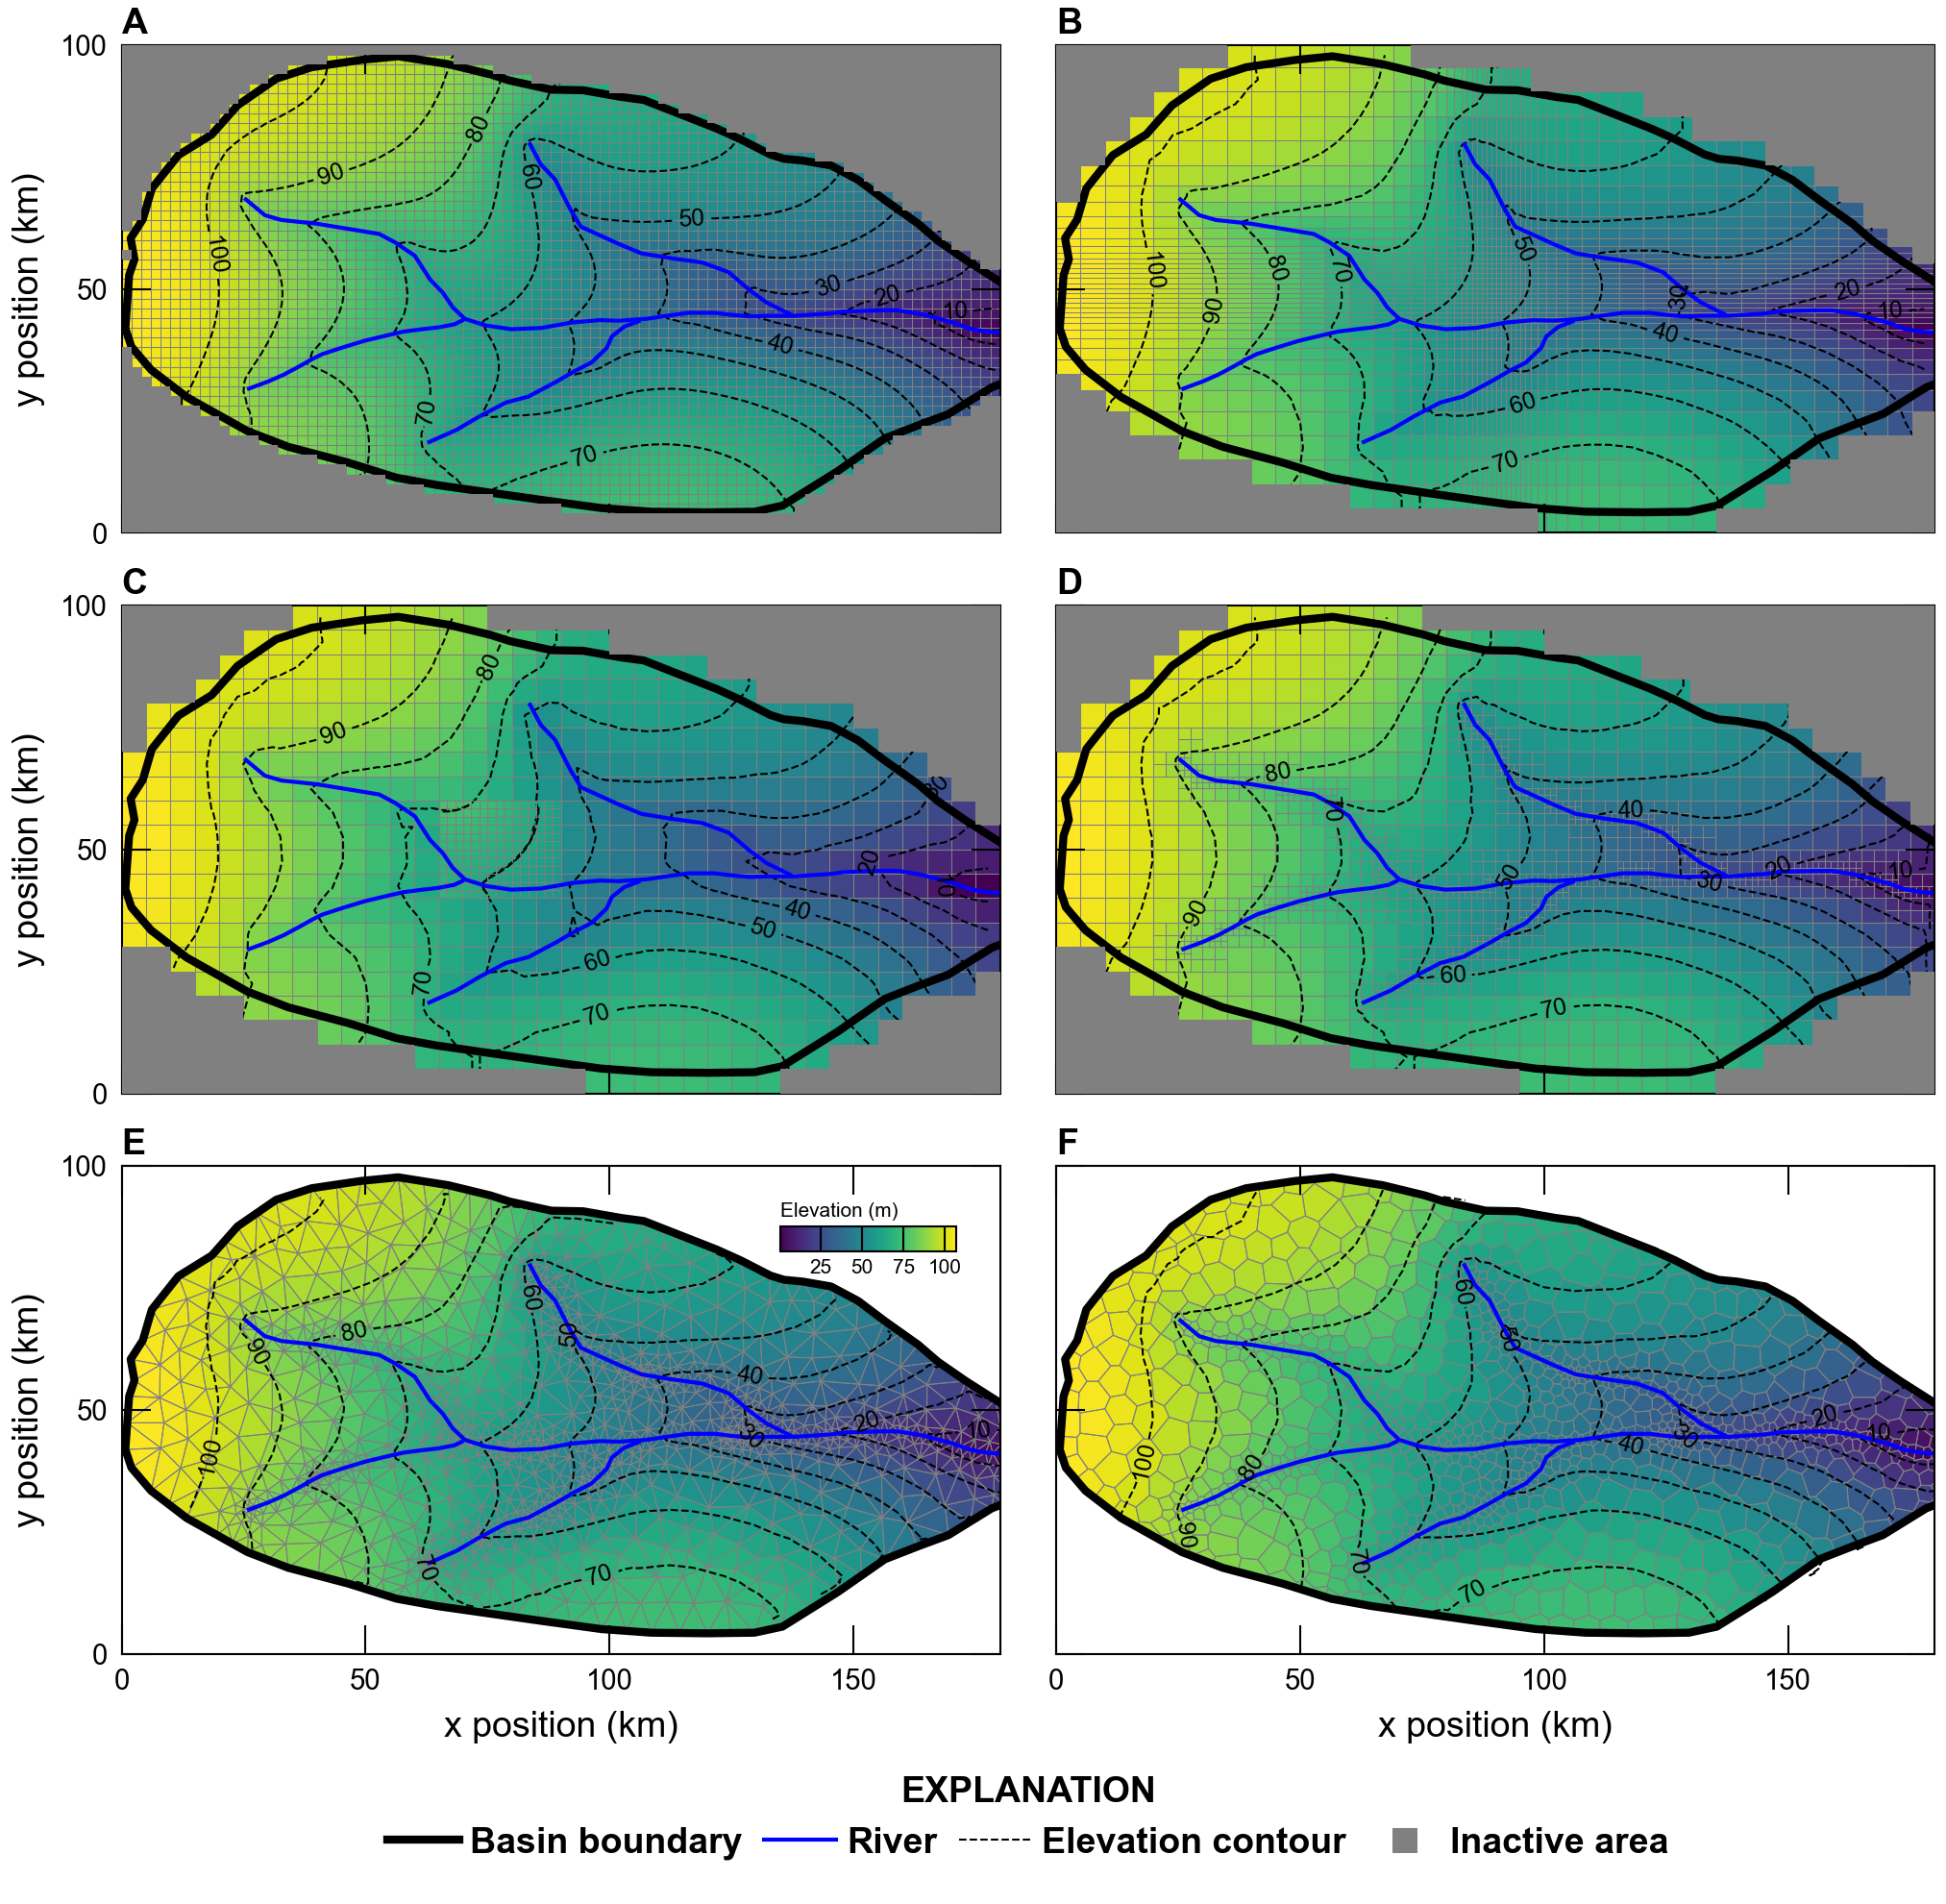
\includegraphics{figures/grids_geoprocessing.png}
	\end{center}
	\caption{Examples of grids that can be generated and processed using FloPy for a hypothetical watershed, including (A) a regular MODFLOW grid with constant and equal row and column spacings, (B) a regular MODFLOW grid with variable row and column spacings, (C) a regular MODFLOW child grid nested within a regular MODFLOW parent grid, (D) a quadtree grid generated with the GRIDGEN program \citep{gridgen} through the FloPy wrapper, (D) a triangular grid generated with the Triangle program \citep{trianglemesh} through the FloPy wrapper, and (E) a Voronoi grid created from the triangular mesh.}\label{fig:grids}
\end{figure}


MODFLOW 6 was developed to natively support multi-model simulations \citep{modflow6framework}. One form of multi-model simulation is a nested grid application in which a more finely discretized child model is embedded within a more coarsely discretized parent model \citep{modflowlgr, vilhelmsen2012evaluation, modflowlgr2}. The use of a locally refined grid (LGR) within a parent grid offers computation benefits in that the additional refinement is targeted to an area of interest. FloPy provides a utility class, called \texttt{Lgr()} for constructing the data required to tightly couple parent and child models within a single MODFLOW 6 simulation.  Figure \ref{fig:grids}C shows two \texttt{StructuredGrid} objects---one object represents the parent model grid and the other represents the nested child grid. The \texttt{Lgr()} defines the connection properties between cells in the parent model and cells in the child model. The utility is general in that the child model can have more layers than the parent model.

FloPy supports management and generation of unstructured grids. Unstructured grids are represented in FloPy as being layered or fully unstructured. A layered grid is one in which the same grid applies to all model layers. An unstructured grid is more general and allows the model grid to change with depth. Layered grids and unstructured grids are stored in FloPy as \texttt{VertexGrid} and \texttt{UnstructuredGrid} objects, respectively.

A layered quadtree grid can be created with FloPy using the \texttt{Gridgen()} utility class, which is a wrapper around the GRIDGEN program \citep{gridgen}. GRIDGEN starts with a regular MODFLOW grid provided by the user. The program then recursively subdivides individual cells that intersect with refinement features into quarters until a maximum level of refinement is met. Refinement features may be points, lines, or polygons. Smoothing is automatically handled so that a cell is connected to no more than two cells in any primary horizontal direction and four cells in the vertical direction.  Figure \ref{fig:grids}D shows an example of a quadtree grid created with GRIDGEN in which a base grid is refined along streams. The following Python code shows the steps for creating the quadtree grid with GRIDGEN.

\begin{python}
>>> sim = flopy.mf6.MFSimulation()
>>> gwf = flopy.mf6.ModflowGwf(sim)
>>> dis6 = flopy.mf6.ModflowGwfdis(gwf, nrow=nrow, ncol=ncol, delr=dy, delc=dx)
>>> g = Gridgen(dis6, model_ws=temp_path)
>>> g.add_refinement_features([[closed_polygon]], "polygon", 0, range(1))
>>> g.add_refinement_features(stream_points, "line", 2, range(1))
>>> g.build(verbose=False)
>>> gridprops_vg = g.get_gridprops_vertexgrid()
>>> quadtree_grid = flopy.discretization.VertexGrid(**gridprops_vg)
\end{python}

FloPy also provides a wrapper utility for the Triangle mesh generation program \citep{trianglemesh}. The FloPy (\texttt{Triangle()}) utility class writes the Triangle program input file, runs the Triangle program, and then loads the triangular mesh. Users provide the maximum area for individual triangles, angle constraints, a polygon describing the model domain, and so forth. Figure \ref{fig:grids}E shows an example of a triangular grid created with the Triangle program. The Python code for creating the triangular grid is shown below.

\begin{python}
>>> tri = flopy.utils.triangle.Triangle(maximum_area=maximum_area, 
... angle=30, nodes=nodes, model_ws=temp_path)
...
>>> tri.add_polygon(boundary_points)
>>> tri.build(verbose=False)
>>> cell2d = tri.get_cell2d()
>>> vertices = tri.get_vertices()
>>> triangular_grid = VertexGrid(vertices=vertices, cell2d=cell2d, 
... idomain=idomain, nlay=nlay, ncpl=tri.ncpl, top=top, botm=botm)
...
\end{python}

A triangular grid can be converted into a Voronoi grid using the \texttt{VoronoiGrid()} utility class within FloPy. This utility class uses SciPy routines \citep{2020SciPy-NMeth} to construct Voronoi polygons around each vertex in the triangular mesh. Figure \ref{fig:grids}F shows an example of a Voronoi grid created from the triangular mesh shown in Figure \ref{fig:grids}D. The steps for creating the voronoi grid from the Triangle object are shown below.

\begin{python}
>>> vor = flopy.utils.voronoi.VoronoiGrid(tri)
>>> gridprops = vor.get_gridprops_vertexgrid()
>>> voronoi_grid = VertexGrid(**gridprops, nlay=nlay, idomain=idomain)
\end{python}

\texttt{StructuredGrid}, \texttt{VertexGrid}, and \texttt{UnstructuredGrid} grid objects have useful properties (\texttt{.property}) and methods (\texttt{.method()}) for accessing or mapping locations on the model grid including: (1) conversion of xy pairs from local to global coordinates (\texttt{.get\_coords()}) and from global to local coordinates (\texttt{.get\_local\_coords()}); (2) getting x, y, and z coordinates for cell centers (\texttt{.xcellcenters}, \texttt{.ycellcenters}, \texttt{.zcellcenters}, and \texttt{.xyzcellcenters}) and vertices (\texttt{.xvertices}, \texttt{.yvertices}, \texttt{.zvertices}, and \texttt{.xyzvertices}); (3) intersecting a list of xy pairs with the grid and returning the appropriate \texttt{cellid} (\texttt{.intersect()}). Other interesting grid object properties and methods include generating a grid object from a MODFLOW 6 binary grid file (\texttt{.from\_binary\_grid\_file()}), calculating the cell thickness for each cell (\texttt{.thick}), and the saturated thickness for each cell (\texttt{.saturated\_thick}).

The ability to develop model grid types using FloPy allows for innovation in the way a study area is discretized in order to tailor the grid to the needs of the study. For example, \cite{Moussa2018} used a voronoi grid to add additional resolution in the vicinity of irrigation wells in the Frenchman Creek Basin in Nebraska, USA to quantify the effects of land-use change and irrigation on streamflow depletion. Furthermore, the ability to develop multi-model simulations using FloPy allows higher-resolution inset models to be added in focused areas. \cite{fienen2022simulation} used focused inset models implicitly coupled to a coarse regional model and solved as a single system of equations to better represent lakes and quantify lake/groundwater interactions in the Central Sands region in Wisconsin, USA. Inset models of lakes in \cite{fienen2022simulation} were developed using \texttt{modflow-setup} \citep{leaf2022modflow}, which relies on FloPy functionality to generate MODFLOW 6 datasets.

\subsection{Geospatial Processing}

Geospatial processing is often a fundamental part of creating a groundwater model. New geospatial processing functionality has been added to FloPy to help users construct models using data from common input sources. The geospatial processing functionality has been implemented to work with the different types of model grids so that it is straightforward to build and construct models with different grid resolutions or grid types. The geospatial processing routines work with all three of the model grid types (\texttt{StructuredGrid}, \texttt{VertexGrid}, and \texttt{UnstructuredGrid}). 

A common geospatial processing task is resampling of raster data onto a model grid. For example, it is often necessary as part of model construction to resample a raster data set of land surface elevation onto a model grid. FloPy includes a new raster sampling utility based on the Rasterio Python package \citep{gillies_2019}. The following Python code demonstrates the steps for resampling an Esri ASCII raster format grid onto a Voronoi grid.

\begin{python}
>>> fine_topo = flopy.utils.Raster.load("./grid_data/fine_topo.asc")
>>> top_vg = fine_topo.resample_to_grid(voronoi_grid, band=fine_topo.bands[0],
... method="linear", extrapolate_edges=True)
...
\end{python}

\noindent The result of raster resampling is a numpy array, equal in size to the number of cells in the Voronoi grid, with an interpolated land surface elevation for each model cell. In this Python code example, the land surface grid was interpolated to the Voronoi grid using a ``linear'' method, however, the method also supports other options (nearest, cubic, mean, median, min, and max) for resampling. The color floods of elevation in Figure \ref{fig:grids} show the results of linear raster resampling for land surface onto a variety of structured and unstructured model grids.

Performing intersections of hydrologic features with the model grid is another common modeling task. FloPy is now equipped with robust and efficient capabilities for intersecting a model grid with points, lines, and polygons. The underlying intersection routines rely on the Shapely Python package \citep{shapely-gillies} to determine intersection properties. When a point or collection of points is intersected with a model grid, the grid intersection routine returns the cells that intersect with the points. When a line or collection of lines is intersected with a model grid, the grid intersection routine returns the cells that intersect with the lines and the lengths of lines within the cell. The line and grid intersection routine also creates and returns individual line segments of the line features within each intersected cell. When a polygon or collection of polygons is intersected with a model grid, the grid intersection routine returns the cells that intersect with the polygons and the polygon area within the cell. The polygon and grid intersection routine also creates and returns individual polygons of the original polygon features within the intersected cells.

The following Python code demonstrates the steps for identifying the grid cells that intersect with a collection of line segments.

% something seems funky with this code example. The grid intersect routine should be able to do this all in one step.
\begin{python}
>>> ixs = flopy.utils.GridIntersect(voronoi_grid, method="vertex")
>>> cellids = []
>>> for points in segments:
...   segment = ixs.intersect(LineString(points), sort_by_cellid=True)
...   cellids += segment["cellids"].tolist()
...
\end{python}

\noindent The result of this code snippet is a list of Voronoi grid cell numbers (called ``cellids'') that intersect with the model grid.  The \texttt{ixs.intersect()} method also returns the \texttt{"lengths"} of the shapelike collection intersecting each cell, the \texttt{"vertices"} corresponding to each cell that intersects a collection of shapelike objects, and a shapely object (\texttt{"ixshape"}) each portion of the original shapelike collection that intersects a cell. Results of the grid intersection for a linear stream network and the six different model grids is shown in Figure \ref{fig:intersections}.

\begin{figure}[ht!]
	\begin{center}
		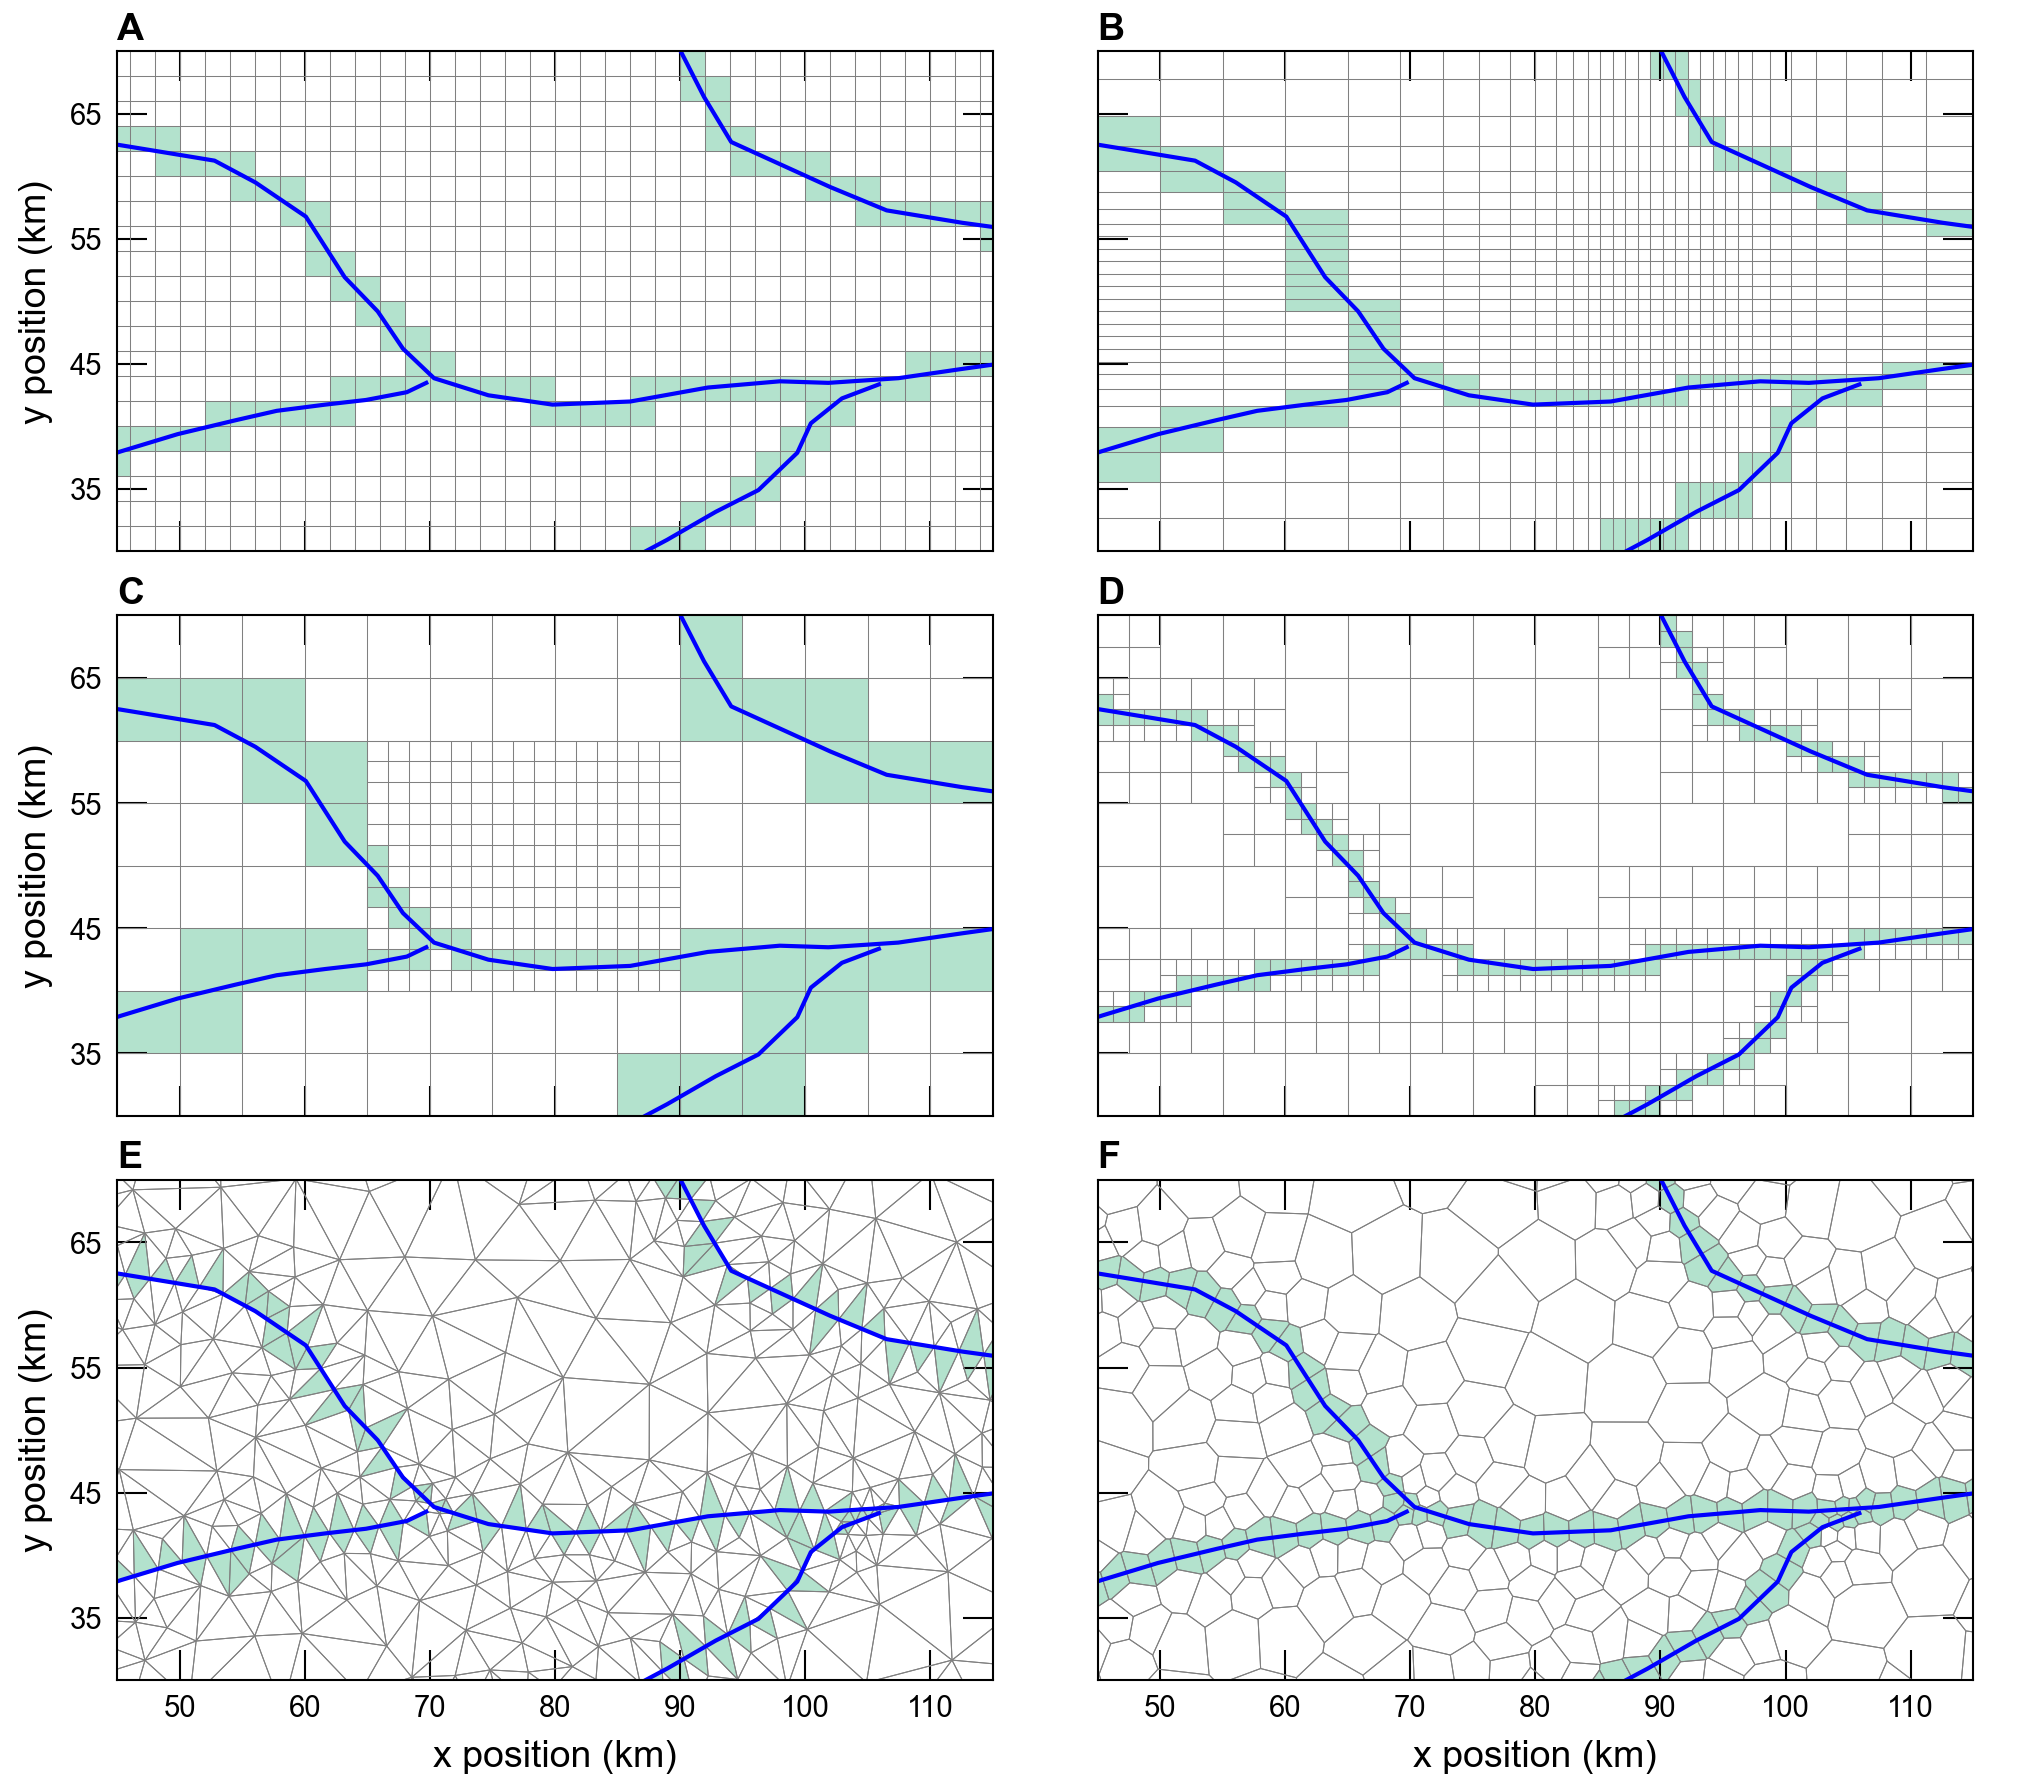
\includegraphics{figures/grids_intersection.png}
	\end{center}
	\caption{Examples of the intersection of a linear stream network with the model grids shown in Figure~\ref{fig:grids}. Intersections were performed using FloPy for (A) a regular MODFLOW grid, (B) a regular MODFLOW grid with variable row and column spacing, (C) a regular MODFLOW child grid nested within a regular MODFLOW parent grid, (D) a quadtree grid, (D) a triangular grid, and (E) a Voronoi grid. Shaded cells represent those cells that intersect with the linear stream network. Individual plots in this figure are centered on the location of the child grid shown in Figure~\ref{fig:grids}C.}
	\label{fig:intersections}
\end{figure}


\subsection{Processing MODFLOW 6 output}

MODFLOW 6 has many different types of output that can be created during a simulation. A GWF Model, for example, can write simulated heads and detailed budget information to binary files. Global model budgets can be written to comma-separated value text files. Some individual GWF and GWT Model advanced stress packages can also write simulated output during a simulation. For example, the Lake (LAK) Package can write simulated lake stages and detailed lake budget information to binary files. Likewise, the Multi-Aquifer Well (MAW) Package can write simulated well head and well budgets to binary files. Recent improvements have been made to FloPy to allows users easier access to simulation results using \texttt{.output} routines. Prior to these improvements, users were required to instantiate head, concentration, and budget file readers using file paths and names in order to access this information. With the \texttt{.output} routines, the readers are automatically generated when called by the user.

The following \texttt{.methods()} syntax shows how a user can discover the type of output information that is available for the specified \texttt{gwf} model.

% not sure where there is a list() object here.
\begin{python}
>>> gwf.output.methods()
['list()', 'zonebudget()', 'budget()', 'budgetcsv()', 'head()']
\end{python}

\noindent The \texttt{.list()} method can be used to get the incremental (\texttt{incremental=True}) or cumulative budget information for the \texttt{gwf} model for a user-specified simulation time, zero-based time step--stress period tuple, or zero-based index. The \texttt{.zonebudget{}} method allows the user to easily build a ZoneBudget6 instance, then run the model, and view output. The \texttt{.budget()} method gives user access to data in binary MODFLOW 6 cell-by-cell budget files. The The \texttt{.budgetcsv()} method gives user access to cumulative and incremental global budget data saved to a comma separated values file. The \texttt{.head()} method gives user access to data in the binary MODFLOW 6 head file.

Similarly, The following \texttt{.methods()} syntax shows how a user can discover the type of output information that is available for advanced stress packages like the LAK package.

\begin{python}
>>> gwf.lak.output.methods()
['zonebudget()', 'budget()', 'budgetcsv()', 'package_convergence()', 'obs()',  'stage()']
\end{python}

\noindent The \texttt{.package\_convergence()} method can be used to get the convergence information for an advanced stress package. The \texttt{.obs()} method can be used to get observation data saved for a model or stress package as a numpy record array or pandas data frame. The \texttt{.stage()} method is the dependent variable for the LAK package and is equivalent to the \texttt{.head()} method for the \texttt{gwf} model. 

\subsubsection{Processing simulated dependent-variable data}

Dependent-variable data (for example, head, stage, or concentration) for a MODFLOW 6 groundwater flow or transport model can be accessed using the \texttt{.output()} method on the GWF or GWT model, respectively. To access the simulated head output, for example, a call can be made to the head reader to retrieve data for a specified simulation time using the \texttt{.get\_data()} method as follows.

\begin{python}
>>> head = gwf.output.head().get_data(totim=1.0)
\end{python}

\noindent In this case, the \texttt{head} variable is a numpy array equal in size to the size of the model grid. Head data can also be accessed for a zero-based time step--stress period tuple 

\begin{python}
>>> head = gwf.output.head().get_data(kstpkper=(0,0))
\end{python}

\noindent or a zero-based index

\begin{python}
>>> head = gwf.output.head().get_data(idx=0)
\end{python}

\noindent in addition providing a user-specified simulation time (\texttt{totim=}). 

\subsubsection{Processing simulated cell-by-cell budget results}

Similar to head output cell-by-cell budget information can be accessed using FloPy. Unlike the simulated head file, the cell-by-cell budget file can have data for more than one item, which can be either arrays or lists of data. The data in the cell-by-cell budget file can be determined using

\begin{python}
>>> gwf.output.budget().list_unique_records()
RECORD           IMETH
----------------------
FLOW-JA-FACE         1
DATA-SPDIS           6
DATA-SAT             6
WEL                  6
DRN                  6
RCHA                 6
EVTA                 6
SFR                  6
LAK                  6
\end{python}

\noindent The \texttt{IMETH} defines if the data is an array (\texttt{IMETH=1}) or is list based (\texttt{IMETH=6}). Cell-by-cell specific-discharge data can be extracted using

\begin{python}
>>> spdis = gwf.output.budget().get_data(totim=1.0, text="DATA-SPDIS")[0]
\end{python}

\noindent Specific-discharge data is returned as a list containing a Numpy record array for the user-specified simulation time (\texttt{totim=}). Like MODFLOW head data, all of the data in the cell-by-cell data file for a user-specified simulation time (\texttt{totim=}), zero-based time step--stress period tuple (\texttt{kstpkper=}), or zero-based index (\texttt{idx=}) can also be extracted. Specific-discharge data can be processed into a form that can be plotted with FloPy using 

\begin{python}
>>> qx, qy, qz = flopy.utils.postprocessing.get_specific_discharge(spdis, gwf, 
... head=head)
\end{python}

\noindent The optional argument \texttt{head=} above sets the specific-discharge in inactive or dry cells to NaN. The \texttt{get\_specific\_discharge()} method also includes functionality to plot specific discharge values at the cell \texttt{"centers"} (default), \texttt{"faces"}, or \texttt{"vertices"}. 

\subsubsection{Performing zone budgets analyses}

\texttt{zonebudget()} output methods are available for both the \texttt{gwf} model and the \texttt{gwf.lak} advanced stress package examples shown above since they both solve a continuity equation. The \texttt{zonebudget()} output method can be used to perform a Zone Budget analysis on the LAK advanced stress package using

\begin{python}
>>> zonbud = gwf.lak.output.zonebudget(zarr)
>>> zonbud.write_input()
>>> zonbud.run_model()
FloPy is using the following executable to run the model: zbud6
                    ZONEBUDGET Version 6
                   U.S. GEOLOGICAL SURVEY
                  VERSION 6.3.0 03/04/2022
.......................................................................
Normal Termination
(True, [])
\end{python}

\noindent \texttt{zarr} in the \texttt{gwf.lak.output.zonebudget()} is a numpy array that defines an integer zone for each lake in the LAK advanced stress package. Zone Budget output can be returned as a numpy record array (\texttt{.get\_budget()} or \texttt{get\_volumetric\_budget()}) or a panda dataframe (\texttt{get\_dataframes()}).

\subsection{Plotting}

Processing output

Maps

\begin{python}
>>> mm = flopy.plot.PlotMapView(model=gwf)
>>> cb = mm.plot_array(head, edgecolor="0.5")
>>> mm.plot_bc("CHD")
>>> mm.plot_vector(qx_top, qy_top, normalize=True)
>>> plt.colorbar(cb, orientation="horizontal");
>>> plt.show()
\end{python}

Cross-sections 

\begin{python}
>>> fx = flopy.plot.PlotCrossSection(model=gwf, 
... line={"line": [(0, 42500), (186801, 42500)]})
...
>>> fx.plot_array(head, head=head)
>>> fx.plot_grid()
>>> plt.show()
\end{python}

%\lipsum[54]

\begin{figure}[ht!]
	\begin{center}
		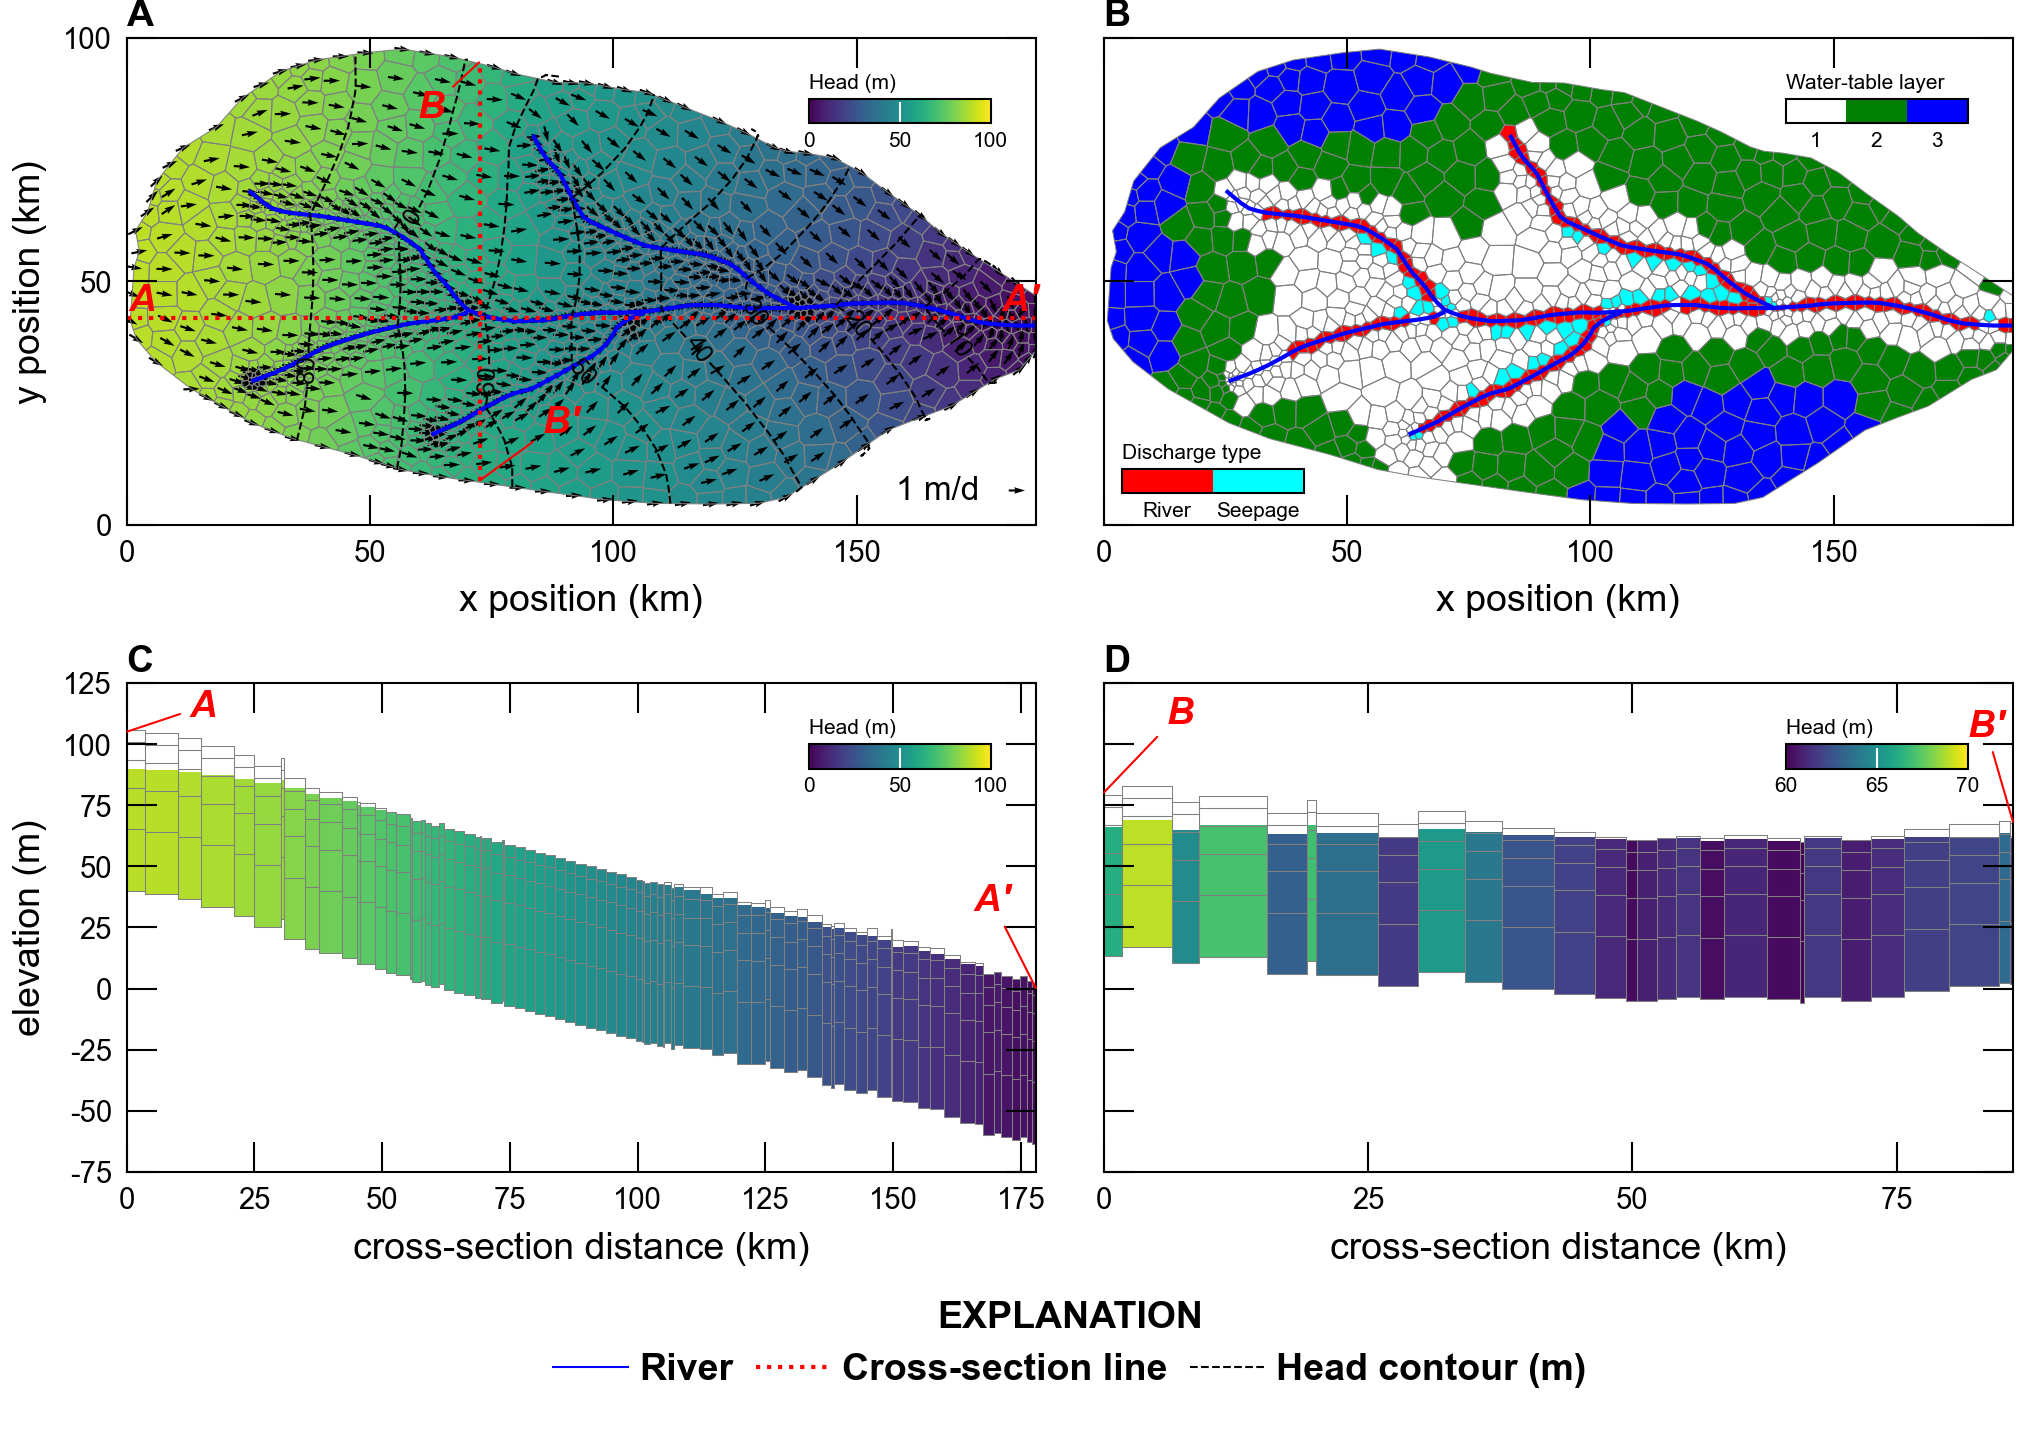
\includegraphics{figures/grids_flopy_plots.png}
	\end{center}
	\caption{FloPy plotting.}
	\label{fig:flopyplots}
\end{figure}

%\lipsum[2-4]

\subsection{Exporting Grid Data to Other Formats}

Model input and output can be exported in a variety of standard formats using the \texttt{export()} method, which is available for FloPy model objects, package objects, and binary dependent-variable (head, concentration, \textit{etc.}) and cell-by-cell output files. Standard output formats that are currently supported include shapefiles \citep{environmental1998esri}, NetCDF files \citep{rew2006netcdf, rew1990netcdf}, and Visualization Tool Kit (VTK) files \citep{schroeder:2006:VTK}.

shapefiles (all grids), VTK (all grids) and NetCDF (structured grids). NetCDF files are being used, for example, by the GWWebFlow viewer? 

\begin{python}
>>> gwf.export("temp_vtk/vtk_smooth", fmt='vtk', smooth=True,
... vertical_exageration=500.0, pvd=True)
...
\end{python}

%\lipsum[2-6]

\begin{figure}[ht!]
	\begin{center}
		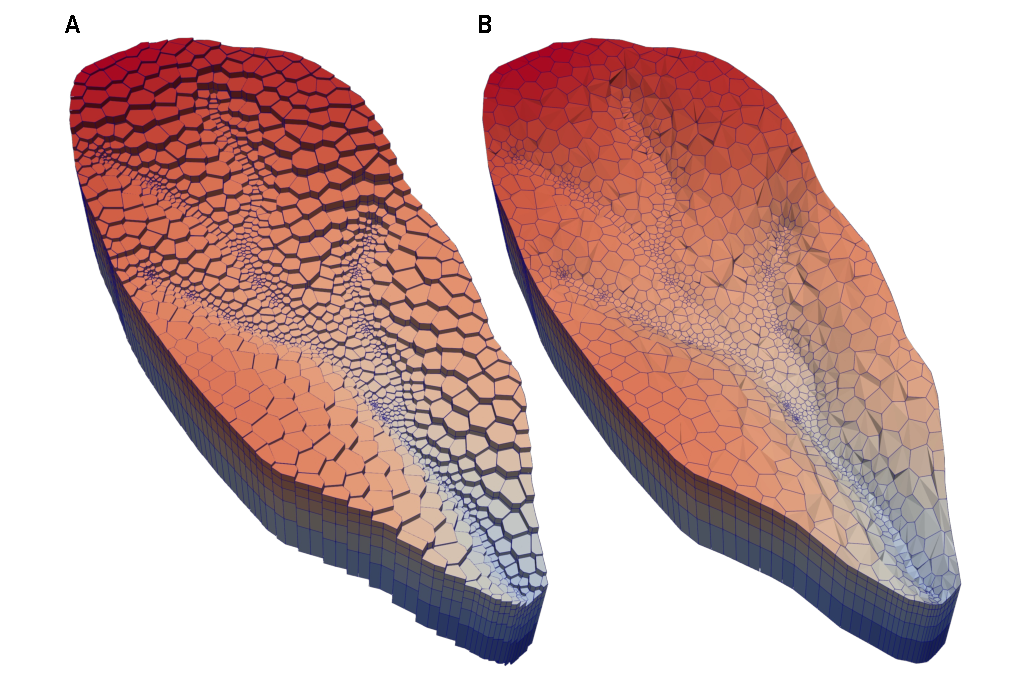
\includegraphics{figures/mf6vtk.pdf}
	\end{center}
	\caption{FloPy export.}
	\label{fig:flopyvtk}
\end{figure}

%\lipsum[2-4]

\section{Scripting MODFLOW 6 Model Development Using Python and FloPy}

\citep{hill1998} presented a synthetic test case (Synthetic Valley) of an undeveloped alluvial valley surrounded by low permeability bedrock. The model included Blue Lake and Straight River surface water features. The model presented in \cite{hill1998} was simulated using MODFLOWP \citep{hill1992computer} using a structured grid with a constant 152.4 meter grid spacing and five model layers. To demonstrate that capabilities of FloPy and MODFLOW 6 we discretized the 6,096 meter x 3,810 meter model domain using a \texttt{VertexGrid} and the discretization by vertices (DISV) package (Figure~\ref{fig:mvgrid}\textit{A}).

%\lipsum[12-18]

\begin{figure}[ht!]
	\begin{center}
		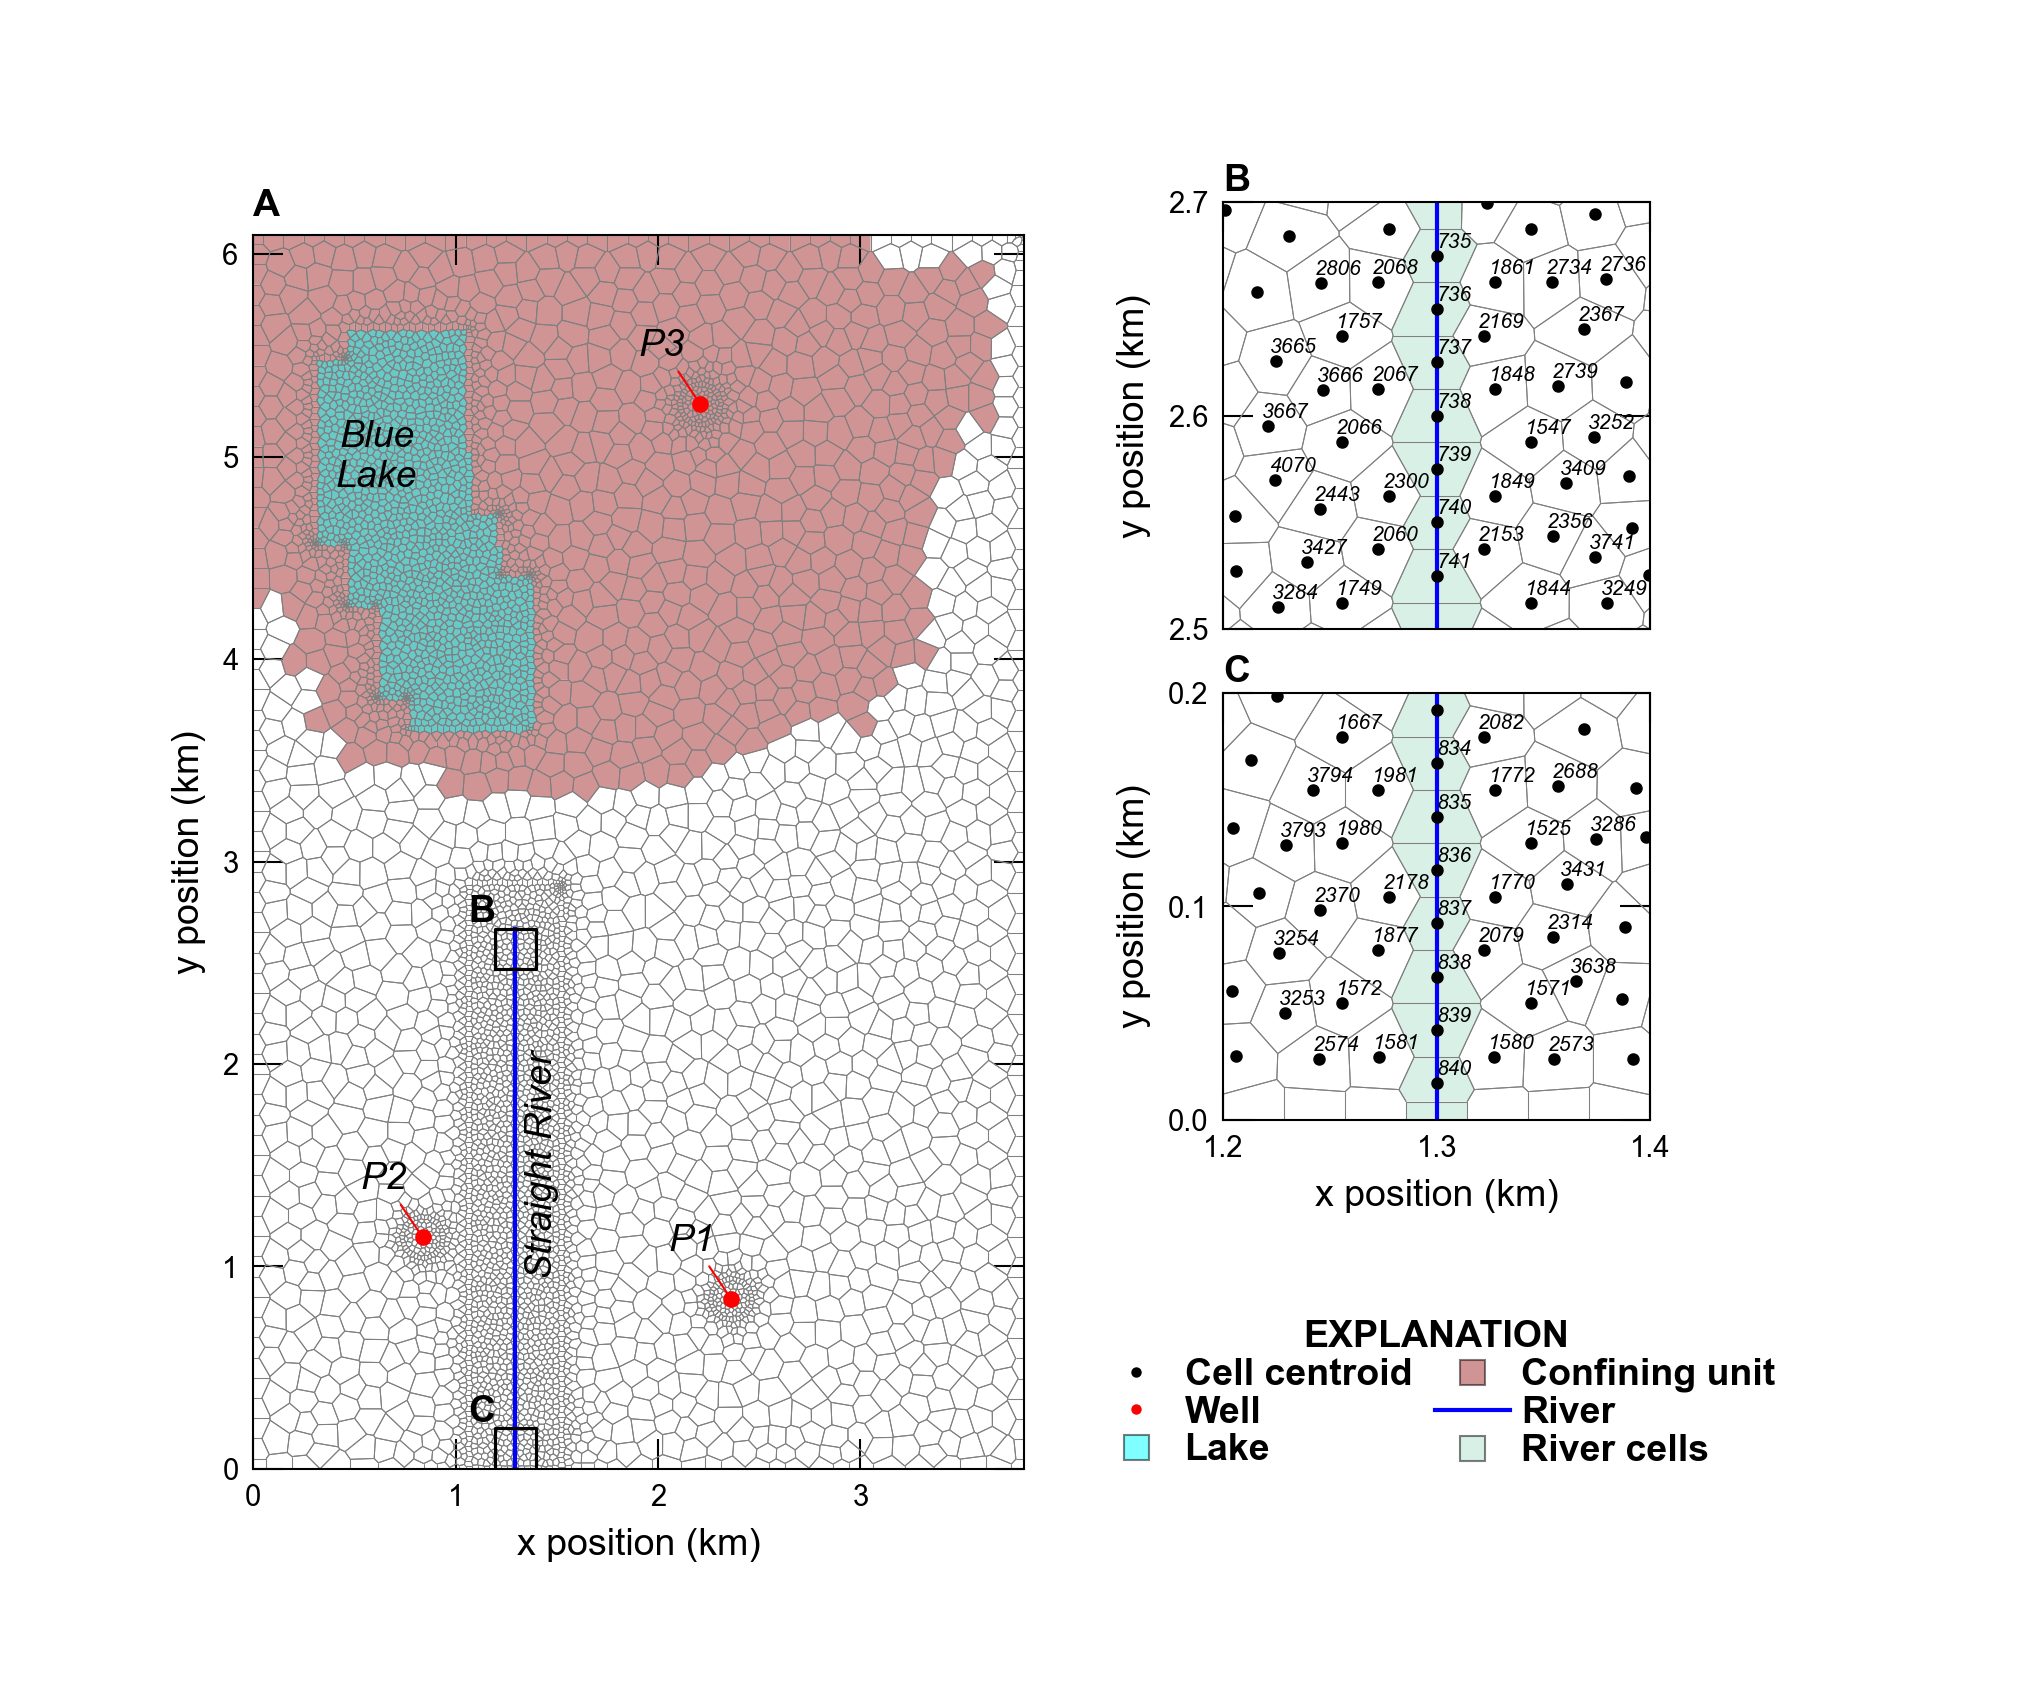
\includegraphics{figures/mv_voronoi_river_discretization.png}
	\end{center}
	\caption{McDonald Valley grid intersections.}
	\label{fig:mvgrid}
\end{figure}

%\lipsum[2-4]

\begin{figure}[ht!]
	\begin{center}
		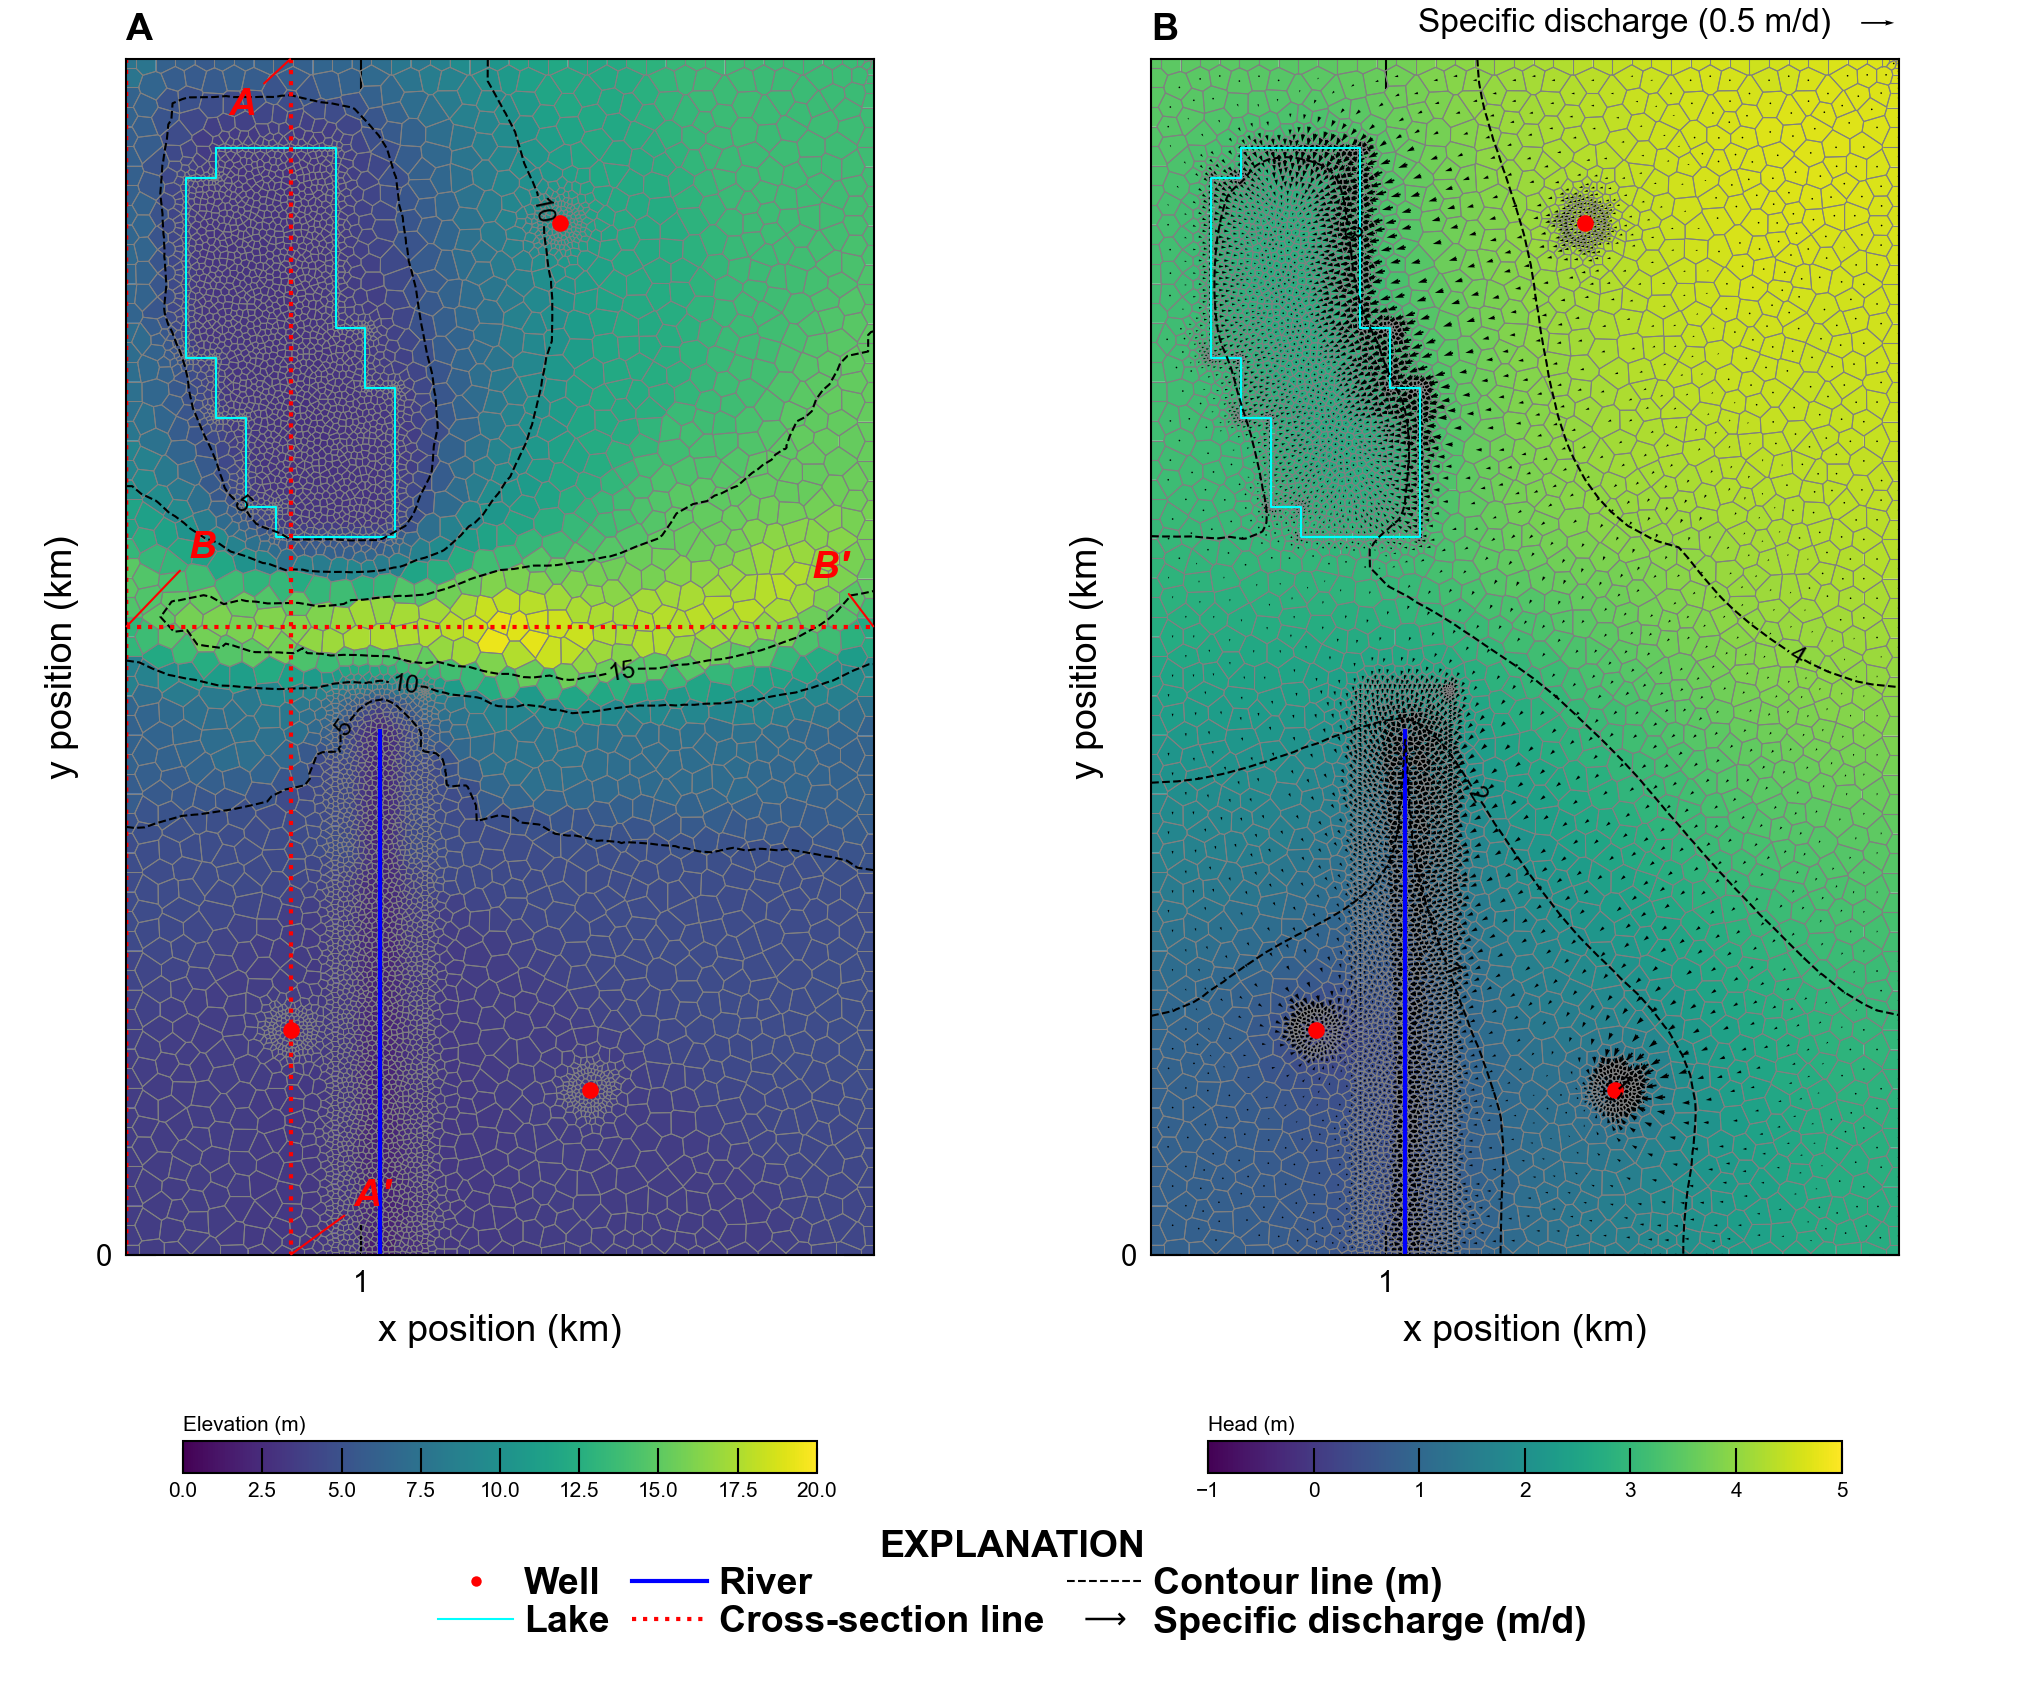
\includegraphics{figures/mv_voronoi_map.png}
	\end{center}
	\caption{McDonald Valley topography and head.}
	\label{fig:mvmap}
\end{figure}

%\lipsum[2-4]

\begin{figure}[ht!]
	\begin{center}
		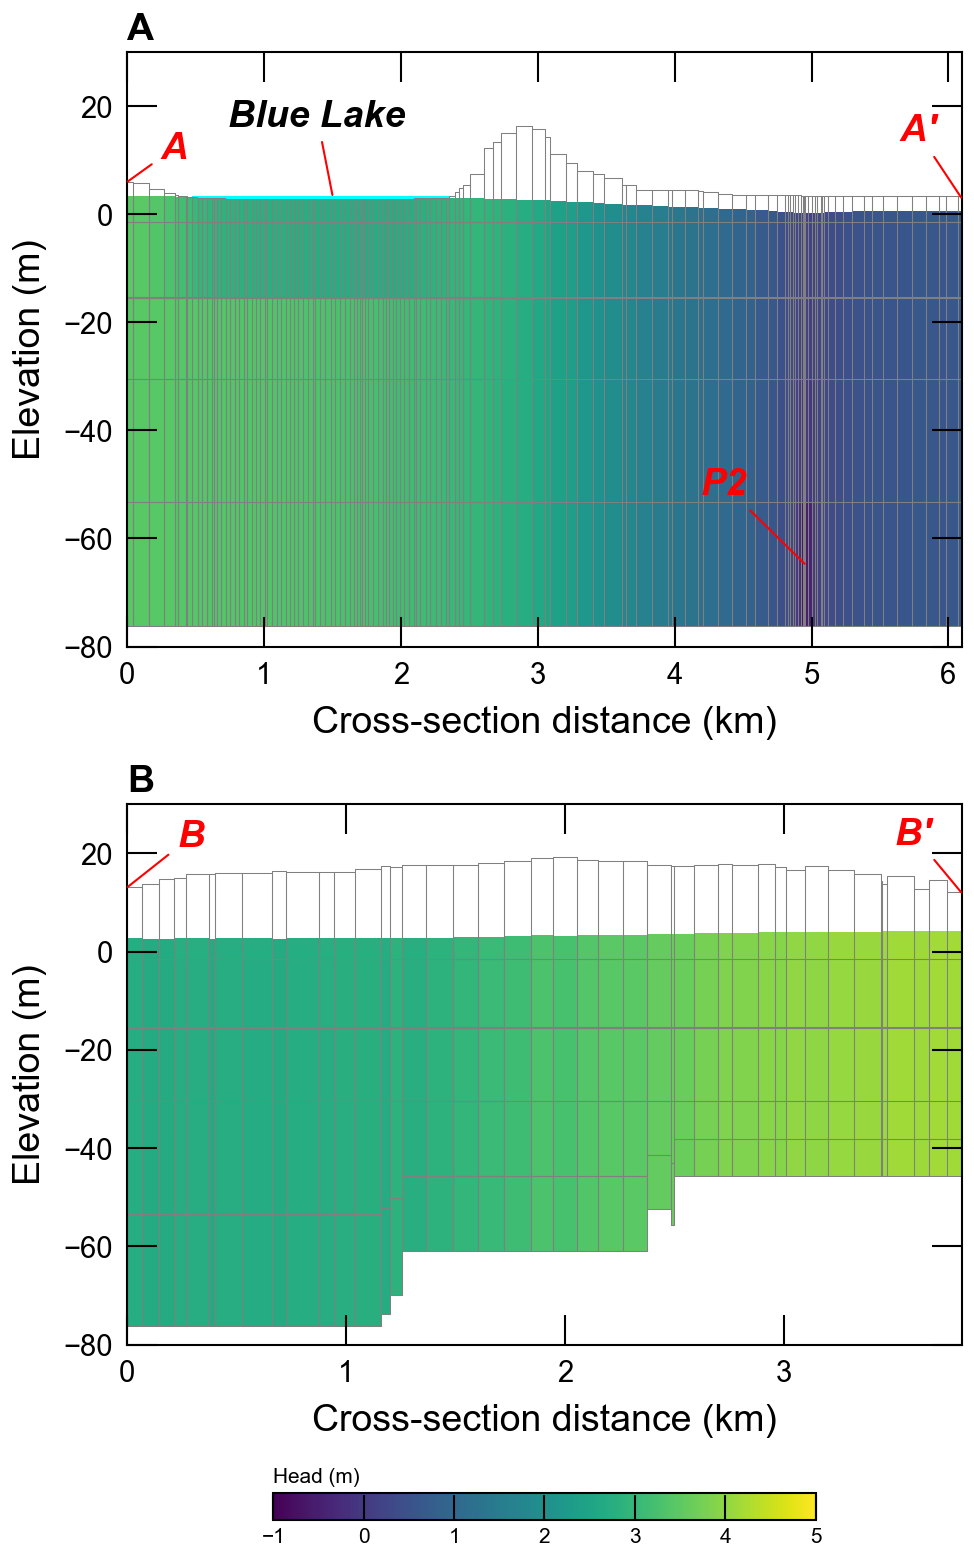
\includegraphics{figures/mv_voronoi_xsection.png}
	\end{center}
	\caption{McDonald Valley topography and head.}
	\label{fig:mvxsection}
\end{figure}

%\lipsum[2-4]

\begin{figure}[ht!]
	\begin{center}
		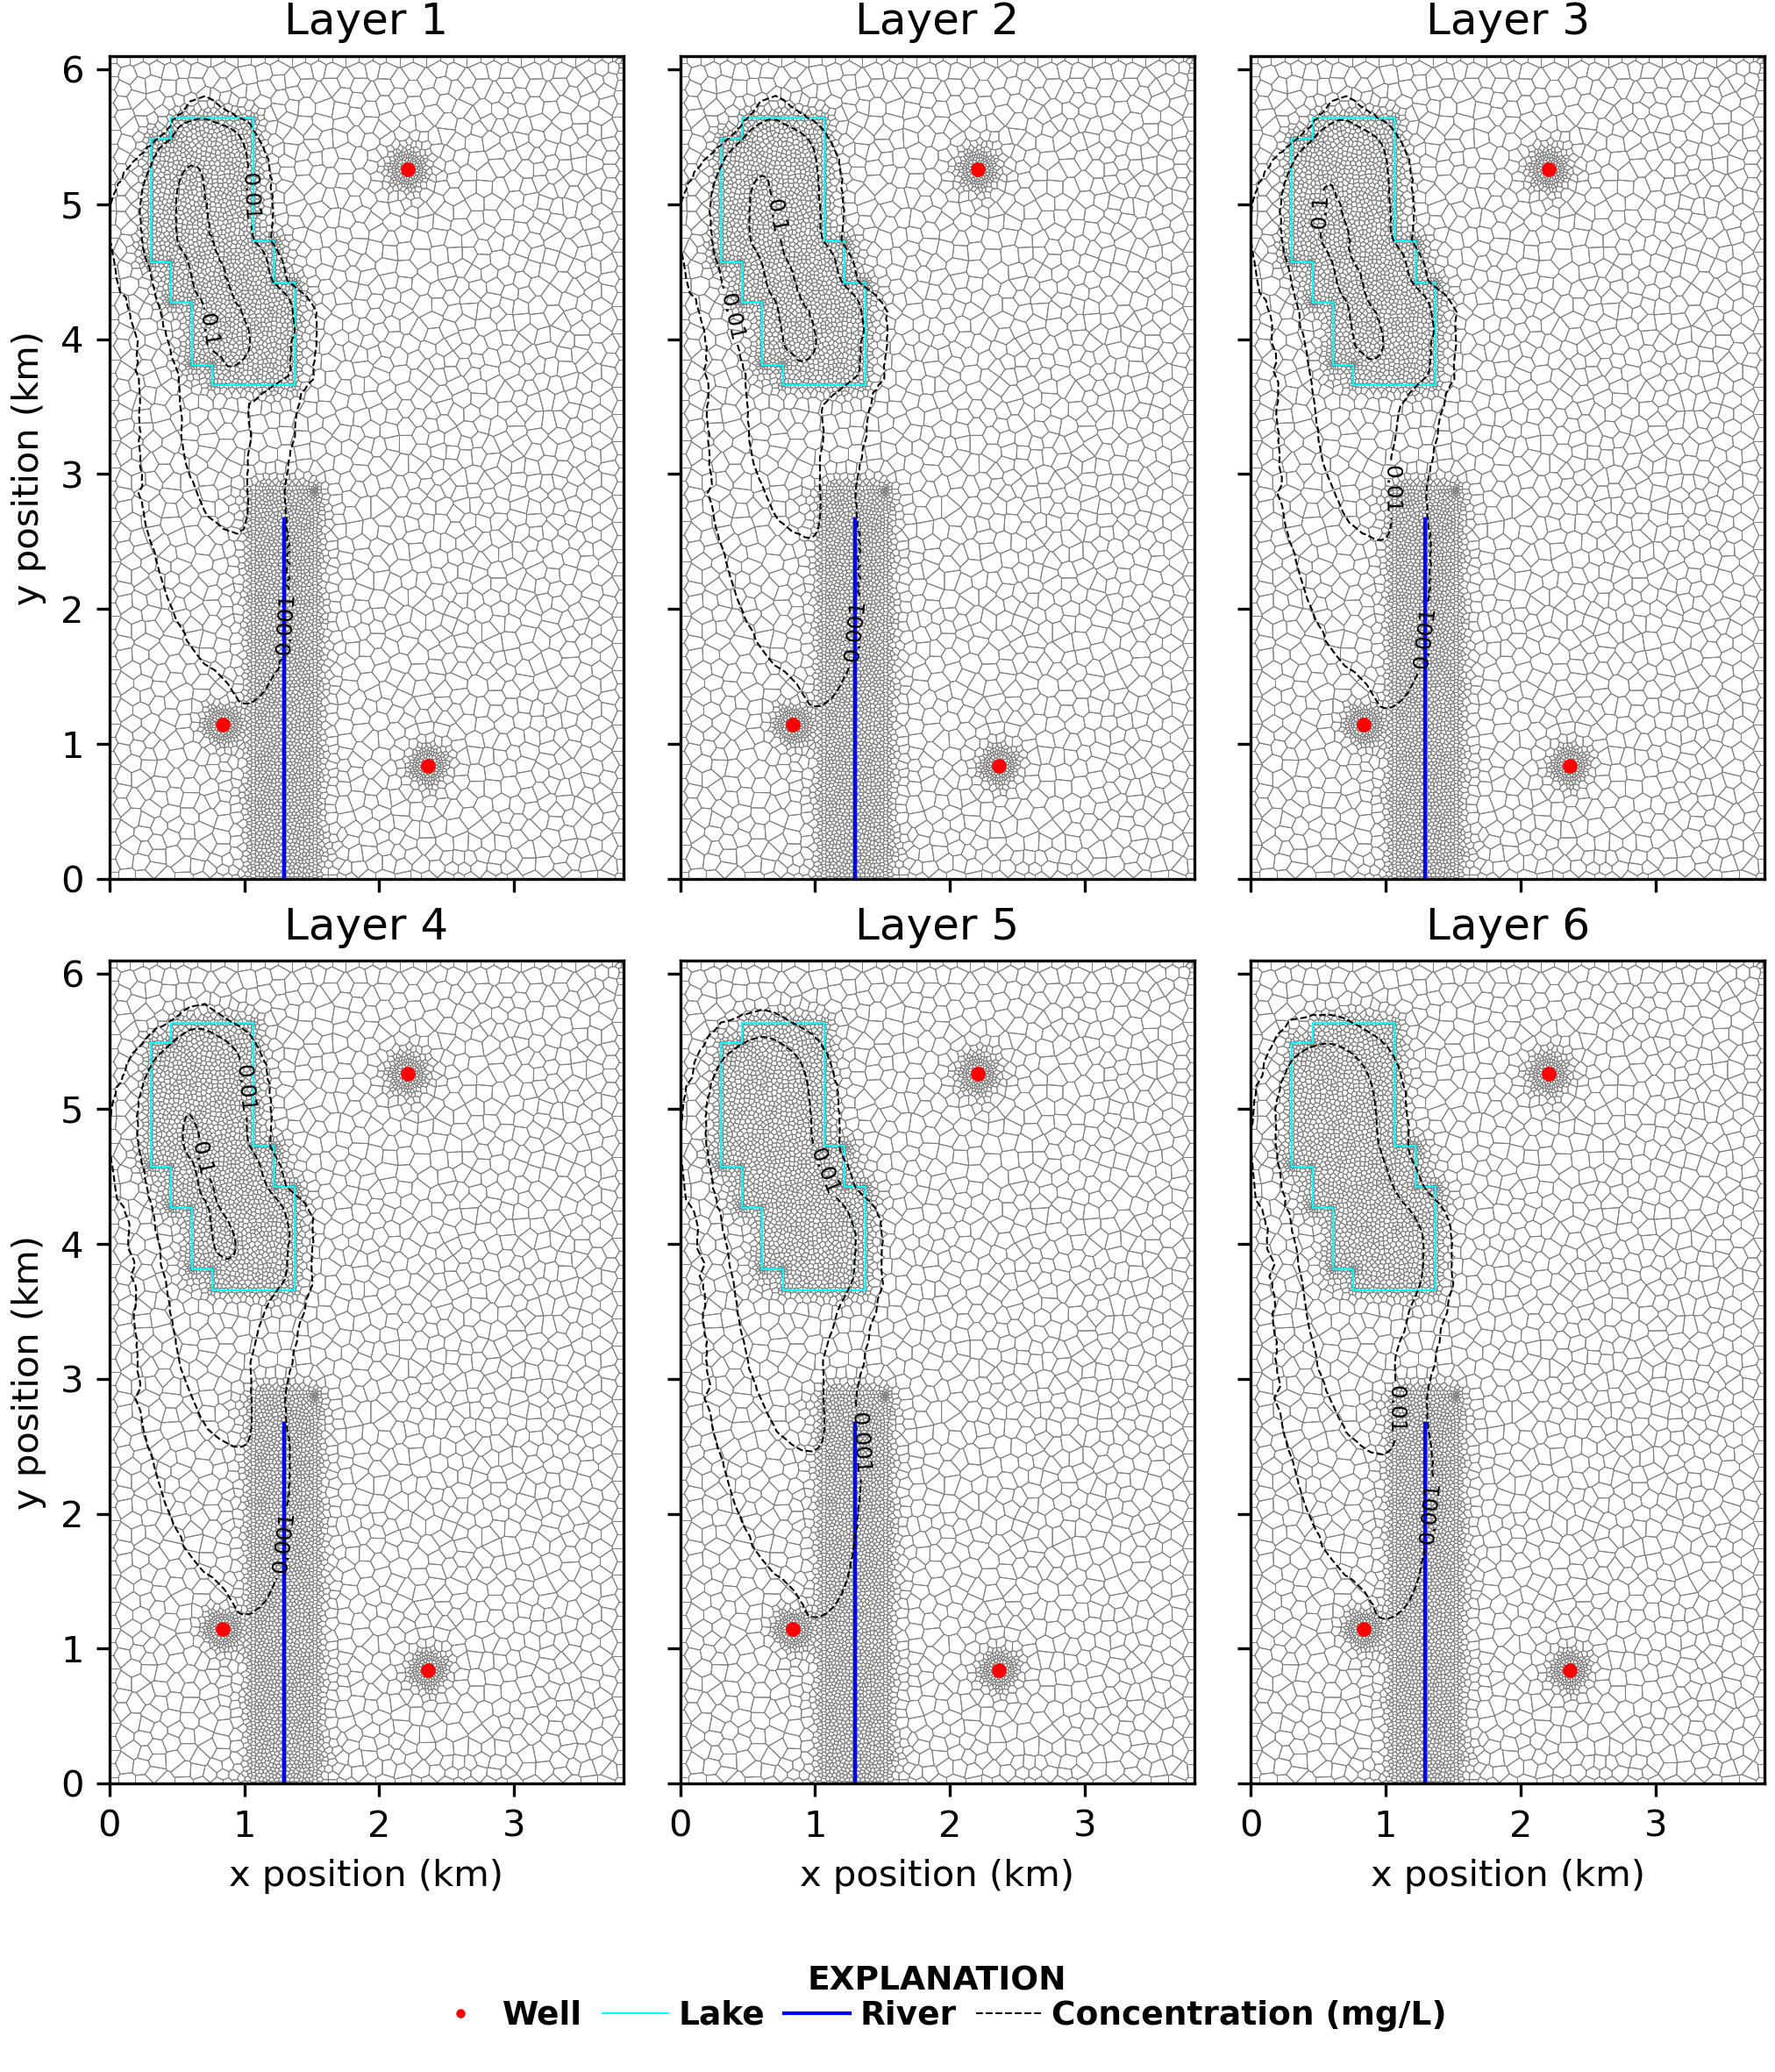
\includegraphics{figures/mv_voronoi_map_concentration.png}
	\end{center}
	\caption{McDonald Valley concentrations.}
	\label{fig:mvxsection}
\end{figure}

%\lipsum[2-4]

\section{Summary and Conclusions}
FloPy is a popular Python package for building, running, and post processing groundwater models. It is open source and developed with input from a growing community of modelers. This paper summarizes important new FloPy capabilities that have been added since the package was first described by \citep{bakker2016scripting}. The new capabilities can be summarized as follows.

\begin{itemize}
\item FloPy supports the creation of many different types of groundwater models, including models that use MODFLOW 6, MODFLOW-2005, MODFLOW-NWT, MODFLOW-USG, MT3D, MT3D-USGS, and SEAWAT. FloPy support for MODFLOW 6 is based on an entirely new approach designed to automatically support all MODFLOW 6 models, packages, and options. The underlying FloPy classes for MODFLOW 6 are programmatically generated from the same input definition files that are used to construct the MODFLOW 6 user guide. This correspondence ensures that the FloPy classes are in direct correspondence with MODFLOW 6 input.
\item FloPy has been extended to support unstructured model grids in addition to regular grids defined by layers, rows, and columns. FloPy has several different routines for creating unstructured grids. FloPy has a wrapper routine around the GRIDGEN program \citep{gridgen}, which can be used to create layered quadtree grids. FloPy also has a wrapper around the Triangle program \citep{trianglemesh}, which can be used to create triangular meshes. A triangular mesh can be converted by FloPy into a Voronoi grid. Grid information is stored for each FloPy model created by the user. This model grid object is used systemically throughout FloPy for geospatial operations, plotting, and exporting model information to supported formats.
\item Geospatial intersections of points, lines, and polygons with model grids and raster resampling onto model grids are common steps in model construction. FloPy fully supports these geospatial operations through its grid intersection and raster resampling routines.
\item Access to model output using FloPy has been simplified for MODFLOW 6 models. 
\item Map and cross section plotting
\item Export to shapefiles, VTK, and NetCDF
\end{itemize}

FloPy makes it possible to construct, and reproduce the construction, of a groundwater model from native data in any format that can be accessed using Python. The robust new features in FloPy allow users to quickly try different model grids, different model spatial and temporal resolution, and different model configurations. 

It is often useful to write a Python script to construct a groundwater model from start to finish. The new geospatial processing routines make it possible to change model resolution as part of the model construction script. This allows one to prototype fast running models with coarse resolution and use finer resolution as the model starts to behave as intended. This workflow also allows one to conduct grid convergence studies to ensure that the grid is not the cause of unintended model behavior.

\section*{Acknowledgments}
The authors gratefully acknowledge the efforts of Mark Bakker and Vincent E.A. Post for initially developing FloPy and their continued efforts improving FloPy. Funding for this research was provided by the Enterprise Capacity (EC) project of the U.S. Geological Survey Integrated Water Prediction program.

\section*{Data Availability Statement}
FloPy is an open source software product and we welcome bug reports, code contributions, or improvements to the documentation from the community. The FloPy python package can be installed using \texttt{conda} or \texttt{pip}. The source code, code documentation, tutorials, and examples can be found in the \href{https://github.com/modflowpy/flopy}{FloPy GitHub repository}. The Synthetic Valley example is available as a \href{https://modflow6-examples.readthedocs.io/en/master/examples.html}{MODFLOW 6 example} and the hypothetical watershed grid examples are available on the \href{https://github.com/modflowpy/flopy/tree/develop/examples/mf6_groundwater_paper}{FloPy GitHub repository}.


\bibliographystyle{groundwater}
\bibliography{flopy}

\end{document}
